%%%%%%%%%%%%%%%%%%%%%%%%%%%%%%%%%%%%%%%%%%%%%%%%%%%%%%%%%%%%%%%%%%%%%%%%%%%%%%%%
%%%%%%%%%%%%%%%%%%%%%%%%%%%%%%%%%%%%%%%%%%%%%%%%%%%%%%%%%%%%%%%%%%%%%%%%%%%%%%%%
%%                                                                            %%
%% thesistemplate.tex version 4.01 (2023/09/21)                               %%
%% The LaTeX template file to be used with the aaltothesis.sty (version 4.00) %%
%% style file.                                                                %%
%% This package requires pdfx.sty v. 1.5.84 (2017/05/18) or newer.            %%
%%                                                                            %%
%% This is licensed under the terms of the MIT license below.                 %%
%%                                                                            %%
%% Written by Luis R.J. Costa.                                                %%
%% Currently developed at Teacher services, Learning Services of Aalto        %%
%% University by Luis R.J. Costa since May 2019.                              %%
%%                                                                            %%
%% Copyright 2017-2021 aaltothesis.cls by Luis R.J. Costa,                    %%
%% luis.costa@aalto.fi.                                                       %%
%% Copyright 2017-2018 Swedish translations in aaltothesis.cls by Elisabeth   %%
%% Nyberg and Henrik Wallén henrik.wallen@aalto.fi.                           %%
%% Finnish documentation in the template opinnatepohja.tex translated from    %%
%% the English template documentation.                                        %%
%% Copyright 2021 English template thesistemplate.tex by Luis R.J. Costa,     %%
%% Maurice Forget, Henrik Wallén.                                             %%
%% Copyright 2018-2022 Swedish template kandidatarbetsbotten.tex by Henrik    %%
%% Wallen.                                                                    %%
%%                                                                            %%
%% Permission is hereby granted, free of charge, to any person obtaining a    %%
%% copy of this software and associated documentation files (the "Software"), %%
%% to deal in the Software without restriction, including without limitation  %%
%% the rights to use, copy, modify, merge, publish, distribute, sublicense,   %%
%% and/or sell copies of the Software, and to permit persons to whom the      %%
%% Software is furnished to do so, subject to the following conditions:       %%
%% The above copyright notice and this permission notice shall be included in %%
%% all copies or substantial portions of the Software.                        %%
%% THE SOFTWARE IS PROVIDED "AS IS", WITHOUT WARRANTY OF ANY KIND, EXPRESS OR %%
%% IMPLIED, INCLUDING BUT NOT LIMITED TO THE WARRANTIES OF MERCHANTABILITY,   %%
%% FITNESS FOR A PARTICULAR PURPOSE AND NONINFRINGEMENT. IN NO EVENT SHALL    %%
%% THE AUTHORS OR COPYRIGHT HOLDERS BE LIABLE FOR ANY CLAIM, DAMAGES OR OTHER %%
%% LIABILITY, WHETHER IN AN ACTION OF CONTRACT, TORT OR OTHERWISE, ARISING    %%
%% FROM, OUT OF OR IN CONNECTION WITH THE SOFTWARE OR THE USE OR OTHER        %%
%% DEALINGS IN THE SOFTWARE.                                                  %%
%%                                                                            %%
%%                                                                            %%
%%%%%%%%%%%%%%%%%%%%%%%%%%%%%%%%%%%%%%%%%%%%%%%%%%%%%%%%%%%%%%%%%%%%%%%%%%%%%%%%
%%                                                                            %%
%%                                                                            %%
%% An example for writting your thesis using LaTeX                            %%
%% Original version and development work by Luis Costa, changes to the text   %%
%% in the Finnish template by Perttu Puska.                                   %%
%% Support for Swedish added 15092014                                         %%
%% PDF/A-b support added on 15092017                                          %%
%% PDF/A-2 support added on 24042018                                          %%
%% Layout design and typesettin changed 15072021                              %%
%%                                                                            %%
%% This example consists of the files                                         %%
%%       thesistemplate.tex (version 4.00) (for text in English)              %%
%%       opinnaytepohja.tex (version 4.00) (for text in Finnish)              %%
%%       kandidatarbetsbotten.tex (version 1.10) (for text in Swedish)        %%
%%       aaltothesis.cls                                                      %%
%%       linediagram.pdf (graphics file)                                      %%
%%       curves.pdf      (graphics file)                                      %%
%%       ledspole.jpg    (graphics file)                                      %%
%%                                                                            %%
%%                                                                            %%
%% Typeset in Linux with                                                      %%
%% pdflatex: (recommended method)                                             %%
%%             $ pdflatex thesistemplate                                      %%
%%             $ pdflatex thesistemplate                                      %%
%%                                                                            %%
%%   The result is the file thesistemplate.pdf that is PDF/A compliant, if    %%
%%   you have chosen the proper \documenclass options (see comments below)    %%
%%   and your included graphics files have no problems.                       %%
%%                                                                            %%
%%                                                                            %%
%% Explanatory comments in this example begin with the characters %%, and     %%
%% changes that the user can make with the character %                        %%
%%                                                                            %%
%%%%%%%%%%%%%%%%%%%%%%%%%%%%%%%%%%%%%%%%%%%%%%%%%%%%%%%%%%%%%%%%%%%%%%%%%%%%%%%%
%%%%%%%%%%%%%%%%%%%%%%%%%%%%%%%%%%%%%%%%%%%%%%%%%%%%%%%%%%%%%%%%%%%%%%%%%%%%%%%%
%%
%% WHAT is PDF/A
%%
%% PDF/A is the ISO-standardized version of the pdf. The standard's goal is to
%% ensure that he file is reproducable even after a long time. PDF/A differs
%% from pdf in that it allows only those pdf features that support long-term
%% archiving of a file. For example, PDF/A requires that all used fonts are
%% embedded in the file, whereas a normal pdf can contain only a link to the
%% fonts in the system of the reader of the file. PDF/A also requires, among
%% other things, data on colour definition and the encryption used.
%% Currently three PDF/A standards exist:
%% PDF/A-1: based on PDF 1.4, standard ISO19005-1, published in 2005.
%%          Includes all the requirements essential for long-term archiving.
%% PDF/A-2: based on PDF 1.7, standard ISO19005-2, published in 2011.
%%          In addition to the above, it supports embedding of OpenType fonts,
%%          transparency in the colour definition and digital signatures.
%% PDF/A-3: based on PDF 1.7, standard ISO19005-3, published in 2012.
%%          Differs from the above only in that it allows embedding of files in
%%          any format (e.g., xml, csv, cad, spreadsheet or wordprocessing
%%          formats) into the pdf file.
%% PDF/A-4: based on PDF 2.0, standard ISO19005-4, published in November 2020.
%%
%% PDF/A-1 files are not necessarily PDF/A-2 -compatible and PDF/A-2 are not
%% necessarily PDF/A-1 -compatible.
%% Standards PDF/A-1, PDF/A-2 and PDF/A-3 have two levels:
%% b: (basic) requires that the visual appearance of the document is reliably
%%    reproduceable.
%% a (accessible) in addition to the b-level requirements, specifies how
%%   accessible the pdf file is to assistive software, say, for the physically
%%   impaired.
%% The PDF/A-4 standard does not have additional levels like in the earlier
%% standards.
%% For more details on PDF/A, see, e.g.,
%% https://www.loc.gov/preservation/digital/formats/fdd/fdd000318.shtml or
%% https://www.pdfa.org/resource/iso-19005-pdfa/
%%
%%
%% WHICH PDF/A standard should my thesis conform to?
%%
%% Either to the PDF/A-1b or the PDF/A-2b standard. If all the figures and
%% graphs used in thesis work do not require transparency features, use either
%% PDF/A-1b or PFDF/A-2b. If you have figures with transparency
%% characteristics, use the PDF/A-2b standard. However, drawing applications
%% often use the transparency parameter, setting it to zero, to specify opacity
%% and get the basic 2-D visualisation. As a result, validation of PDF/A-1b
%% will fail. Use PDF/A-2b if PDF/A-1b validation fails.
%% Do not use the PDF/A-3b standard for your thesis.
%% The font to be used are specified in this templatenand they should not be
%% changed. In addition to not adhering to Aalto's visual guidelines, you may
%% have difficulties in producing a PDF/A-compliant PDF.
%%
%%
%% Validate your PDF/A file at https://www.pdf-online.com/osa/validate.aspx
%%
%%
%% WHAT graphics format can I use to produce my PDF/A compliant file?
%%
%% When using pdflatex to compile your work, favour the use of pdf, but you can
%% use the jpg or png format especially for photographs. You will have PDF/A
%% compliance problems with figures in pdf if the fonts are not embedded in the
%% pdf file.
%% If you choose to use latex to compile your work, the only acceptable file
%% format for your figure is eps. DO NOT use the ps format for your figures.

%% USE one of the following three \documentclass set-ups:
%% * the first when using pdflatex to directly typeset your document in the
%%   chosen pdf/a format for online publishing (centred page layout),
%% * the second for one-sided printing your thesis with the layout (wide left
%%   margin), or
%% * the third for two-sided printing.
%%
\documentclass[english, 12pt, a4paper, elec, utf8, a-2b, online]{aaltothesis}
%\documentclass[english, 12pt, a4paper, elec, utf8, a-2b, print]{aaltothesis}
%\documentclass[english, 12pt, a4paper, elec, utf8, a-2b, print, twoside]{aaltothesis}

%% Use the following options in the \documentclass macro above:
%% your school: arts, biz, chem, elec, eng, sci
%% the character encoding scheme used by your editor: utf8, latin1
%% thesis language: english, finnish, swedish
%% make an archiveable PDF/A-1b or PDF/A-2b compliant file: a-1b, a-2b
%%                    (with pdflatex, a normal pdf containing metadata is
%%                     produced without the a-*b option)
%% typset for online document or print on paper: online, print
%%        online: typeset in symmetric layout and blue hypertext for online
%%                publishing
%%        print: typeset in a symmetric layout and black hypertext for printing
%%               on paper
%%          two-side printing: twoside (default is one-sided printing)
%%               typeset in a wide margin on the binding side of the page and
%%               black hypertext. Use with print only.
%%

%% Use one of these if you write in Finnish (or use the Finnish template
%% opinnaytepohja.tex)
%\documentclass[finnish, 12pt, a4paper, elec, utf8, a-1b, online]{aaltothesis}
%\documentclass[finnish, 12pt, a4paper, elec, utf8, a-1b, print]{aaltothesis}
%\documentclass[finnish, 12pt, a4paper, elec, utf8, a-1b, print, twoside]{aaltothesis}

%% Use one of these if you write in Swedish (or use the Swedish template
%% kandidatarbetsbotten.tex)
%\documentclass[swedish, 12pt, a4paper, elec, utf8, a-2b, online]{aaltothesis}
%\documentclass[swedish, 12pt, a4paper, elec, utf8, a-2b]{aaltothesis}
%\documentclass[swedish, 12pt, a4paper, elec, dvips, online]{aaltothesis}

%% FOR USERS OF AMS PACKAGES:
%% * newtxmath used in this template loads amsmath, so
%%   you needn't load it. If you want to use options in amsmath, load it here,
%%   before \setupthesisfonts below to pass the options to amsmath.
%% * If you want to use amsthm, load it here before \setupthesisfonts to avoid
%%   a clash with newtxmath.
%% * If using amsmath with options and you want to use amsthm, load amsthms
%%   after amsmath, as described in the amsthm documentation.
%% * Don't use amsbsym or amsfonts. The symbols [and macros] there are defined in
%%   newtxmath and so clash if used.
%\usepackage[options]{amsmath}
%\usepackage{amsthm}

%% DO NOT MOVE OR REMOVE \setupthesisfonts
\setupthesisfonts

%%
%% Add here the packges you need
%%
\usepackage{graphicx}
\usepackage{textcomp}
\usepackage{minted}
\usepackage{subcaption}

\usepackage[version=4]{mhchem}
% \usepackage{fontspec}


\usepackage[printonlyused,withpage]{acronym}


%% For tables that span multiple pages; used to split a paraphrasing example in
%% the appendix. If you don't need it, remove it.
\usepackage{longtable}

%% A package for generating Creative Commons copyright terms. If you don't use
%% the CC copyright terms, remove it, since otherwise undesired information may
%% be added to this document's metadata.
\usepackage[type={CC}, modifier={by-nc-sa}, version={4.0}]{doclicense}
%% Find below three examples for typesetting the CC license notice.


%% Edit to conform to your degree programme
%% Capitalise the words in the name of the degree programme: it's a name
\degreeprogram{Data Science}
%%

%% Your major
%%
\major{ICT Innovation}
%%

%% Choose one of the three below
%%
%\univdegree{BSc}
\univdegree{MSc}
%\univdegree{Lic}
%%

%% Your name (self explanatory...)
%%
\thesisauthor{Gabriel Gomes Ziegler}
%%

%% Your thesis title and possible subtitle comes here and possibly, again,
%% together with the Finnish or Swedish abstract. Do not hyphenate the title
%% (and subtitle), and avoid writing too long a title. Should LaTeX typeset a
%% long title (and/or subtitle) unsatisfactorily, you might have to force a
%% linebreak using the \\ control characters. In this case...
%% * Remember, the title should not be hyphenated!
%% * A possible 'and' in the title should not be the last word in the line; it
%%   begins the next line.
%% * Specify the title (and/or subtitle) again without the linebreak characters
%%   in the optional argument in box brackets. This is done because the title
%%   is part of the metadata in the pdf/a file, and the metadata cannot contain
%%   linebreaks.
%%
\thesistitle{Automating Information Extraction from Non-Standard Financial Reports Using Large Language Models}
%\thesistitle[Title of the thesis]{Title of\\ the thesis}
%%
%% Either remove or leave \thesissubtitle{} empty if you don't use it
%%
\thesissubtitle{Enhancing Efficiency through Format-Aware Extraction with Large Language Models}
%\thesissubtitle[Subtitle of the thesis]{Subtitle of\\ the thesis}
%\thesissubtitle{}

%%
\place{Espoo}
%%

%% The date for the bachelor's thesis is the day it is presented
%%
\date{21 September 2023}
%%

%% Thesis supervisor
%% Note the "\" character in the title after the period and before the space
%% and the following character string.
%% This is because the period is not the end of a sentence after which a
%% slightly longer space follows, but what is desired is a regular interword
%% space.
%%
\supervisor{Prof.\ Bo Zhao}
%%

%% Advisor(s)---two at the most---of the thesis. Check with your supervisor how
%% many official advisors you can have.
%%
\advisor{MS Liliya Shakhpazyan (MSc)}
%%

%% If you do your thesis work in a company of other institute, give the name of
%% the company or instution here. Otherwise, leave the macro empty, comment it
%% out, or remove it. This will remove this field from the abstract page.
%%
\collaborativepartner{Datia}
%%

%% Aaltologo: syntax:
%% \uselogo{?|!|''}
%% The logo language is set to be the same as the thesis language.
%%
%\uselogo{?}
%\uselogo{!}
\uselogo{''}
%%

%%%%%%%%%%%%%%%%%%               COPYRIGHT TEXT               %%%%%%%%%%%%%%%%%%
%%%%%%%%%%%%%%%%%%%%%%%%%%%%%%%%%%%%%%%%%%%%%%%%%%%%%%%%%%%%%%%%%%%%%%%%%%%%%%%%

%% Copyright of a work is with the creator/author of the work regardless of
%% whether the copyright mark is explicitly in the work or not. You may, if you
%% wish---we encourage you to do so---publish your work under a Creative
%% Commons license (see creativecommons.org), in which case the license text
%% must be visible in the work. Write here the copyright text you want using the
%% macro \copyrighttext, which writes the text into the metadata of the pdf file
%% as well.
%%
%% Syntax:
%% \copyrigthtext{metadata text}{text visible on the page}
%%
%% CHOOSE ONE OF THE COPYRIGHT NOTICE STYLES BELOW.
%% IF USING THE CC TERMS, CHOOSE THE LICENSE YOU WANT TO USE.
%% The different CC licenses are listed at
%% https://creativecommons.org/about/cclicenses/.
%% If you use the icons from the dolicense.sty package, add the package above
%% (\usepackage{dolicense}).
%% IMPORTANT NOTE!! Manually write the CC text in the \copyrighttext metadata
%% text field.
%%
%% NOTE: In the macros below, the text written in the metadata must have a
%% \noexpand macro before the \copyright special character. When not in pdf/a
%% mode (i.e. a-1b or a-2b are not specified in \documentclass), two \noexpands
%% are required in the metadata text to correctly render the copyright mark in
%% the pdf metadata. In pdf/a mode one \noexpand suffices.
%%
%% EXAMPLE OF PLAIN COPYRIGHT TEXT
%% The macros \copyright and \year below must be separated by the \ character
%% (space chacter) from the text that follows. The macros in the argument of the
%% \copyrighttext macro automatically insert the year and the author's name.
%% (Note! \ThesisAuthor is an internal macro of the aaltothesis.cls class file).
%%
%\copyrighttext{Copyright \noexpand\textcopyright\ \number\year\ \ThesisAuthor}
%{Copyright \textcopyright{} \number\year{} \ThesisAuthor}
%%
%% Of course, the same text could have simply been written as
%% \copyrighttext{Copyright \noexpand\copyright\ 2018 Eddie Engineer}
%% {Copyright \copyright{} 2022 Eddie Engineer}
%%
%% EXAMPLES OF CC LICENSE: different ways to display the same license
%% 1. A simple Creative Commons license text with a link to the copyright notice:
%\copyrighttext{\noexpand\textcopyright\ \number\year. This work is
%	licensed under a CC BY-NC-SA 4.0 license.}{\textcopyright{}
%	\number\year. This work is licensed under a
%	\href{https://creativecommons.org/licenses/by-nc-nd/4.0/}{CC BY-NC-SA 4.0}
%	license.}
%
%% To get the URL of the license of your choice, go to
%% https://creativecommons.org/about/cclicenses/, click on the chosen license
%% you want to use, and copy-and-paste the URL in the macro \href above.
%%
%% 2. A short Creative Commons license text containing the respective CC icons
%% (requires the package dolicense.sty to be added in the preamble as done
%% above) and a link to the corresponding Creative Commons license webpage (see
%% the dolicense package documentation for other license icons):
%\copyrighttext{\noexpand\textcopyright\ \number\year. This work is licensed
%	under a CC BY-NC-SA 4.0 license.}{
%	\parbox{95mm}{\noindent\textcopyright\ \number\year. \doclicenseText}
%	\hspace{1em}\parbox{35mm}{\doclicenseImage}
%}
%%
%% 3. An expanded Creative Commons license text containing the respective CC
%% icons text and as generated by the dolicense.sty package (the license is set
%% via package options in \usepackage[options]{dolicense} above; see the
%% dolicense package documentation for other license texts and icons):
\copyrighttext{\noexpand\textcopyright\ \number\year. This work is
    licensed under a Creative Commons "Attribution-NonCommercial-ShareAlike 4.0
    International" (BY-NC-SA 4.0) license.}{\noindent\textcopyright\ \number
    \year \ \doclicenseThis}
%%%%%%%%%%%%%%%%%%%%%%%%%%%%%%%%%%%%%%%%%%%%%%%%%%%%%%%%%%%%%%%%%%%%%%%%%%%%%%%%


%% The English abstract:
%% All the details (name, title, etc.) on the abstract page appear as specified
%% above.
%% Thesis keywords:
%% Note! The keywords are separated using the \spc macro
%%
\keywords{For keywords choose\spc concepts that are\spc central to your\spc
thesis}
%%

%% The abstract text. This text in one paragraph is included in the metadata of
%% the pdf file as well as the abstract page. To have paragraphs in your
%% abstract rewrite it in the abstarct environment as described below.
%%
\thesisabstract{%
The abstract is a short description of the essential contents of the thesis
usually in one paragraph: what was studied and how and what were the main
findings. For a Finnish thesis, the abstract should be written in both Finnish
and English; for a Swedish thesis, in Swedish and English. The abstracts for
English theses written by Finnish or Swedish speakers should be written in
English and either in Finnish or in Swedish, depending on the student’s language
of basic education. Students educated in languages other than Finnish or Swedish
write the abstract only in English. Students may include a second or third
abstract in their native language, if they wish.
The abstract text of this thesis is written on the readable abstract page as
well as into the pdf file’ metadata via the thesisabstract macro (see the
comment in the TeX file). Write here the text that goes into the metadata. The
metadata cannot contain special characters, linebreak or paragraph break
characters, so these must not be used here. If your abstract does not contain
special characters and it does not require paragraphs, you may take advantage of
the abstracttext macro (see the comment in the TeX file below). Otherwise, the
metadata abstract text must be identical to the text on the abstract page.
}

%% You can prevent LaTeX from writing into the xmpdata file (it contains all the
%% metadata to be written into the pdf file) by setting the writexmpdata switch
%% to 'false'. This allows you to write the metadata in the correct format
%% directly into the file thesistemplate.xmpdata.
%\setboolean{writexmpdatafile}{false}


%% All that is printed on paper starts here
%%
\begin{document}

%% Create the coverpage
%%
\makecoverpage

%% Typeset the copyright text.
%% If you wish, you may leave out the copyright text from the human-readable
%% page of the pdf file. This may seem like a attractive idea for the printed
%% document especially if "Copyright (c) yyyy Eddie Engineer" is the only text
%% on the page. However, the recommendation is to print this copyright text.
%%
\makecopyrightpage

\clearpage
%% Note that when writing your thesis in English, place the English abstract
%% first followed by the possible Finnish or Swedish abstract.

%% Abstract text
%% All the details (name, title, etc.) on the abstract page appear as specified
%% above. Add your abstarct text with paragraphs here to have paragraphs in the
%% visible abstract page. Nonetheless, write the abstarct text without
%% paragraphs in the macro \thesismacro so that it is added to the metadata as
%% well.
%%
\begin{abstractpage}[english]
  The abstract is a short description of the essential contents of the thesis,
  usually in one paragraph: what was studied and how and what were the main
  findings.

  For a Finnish thesis, the abstract should be written in both Finnish and
  English; for a Swedish thesis, in Swedish and English. The abstracts for
  English theses written by Finnish or Swedish speakers should be written in
  English and either in Finnish or in Swedish, depending on the student’s
  language of basic education. Students educated in languages other than Finnish
  or Swedish write the abstract only in English. Students may include a second
  or third abstract in their native language, if they wish.

  The abstract text of this thesis is written on the readable abstract page as
  well as into the pdf file’ metadata via the \verb+\thesisabstract+ macro
  (see comment in this \TeX{} file above). Write here the text that goes onto
  the readable abstract page. You can have special characters, linebreaks, and
  paragraphs here. Otherwise, this abstract text must be identical to the
  metadata abstract text.

  If your abstract does not contain special characters and it does not require
  paragraphs, you may take advantage of the \verb+\abstracttext+ macro (see the
  comment in this \TeX{} file below).
\end{abstractpage}

%% The text in the \thesisabstract macro is stored in the macro \abstractext, so
%% you can use the text metadata abstract directly as follows:
%%
%\begin{abstractpage}[english]
%	\abstracttext{}
%\end{abstractpage}

%% Force a new page so that the possible Finnish or Swedish abstract does not
%% begin on the same page
%%
\newpage
%%
%% Abstract in Finnish. Delete if you don't need it.
%%
%% Respecify those fields that differ from the earlier specification or simply
%% respecify all fields.
\thesistitle{Opinnäyteen otsikko}
\thesissubtitle{Opinnäytteen mahdollinen alaotsikko}
\supervisor{Prof.\ Pirjo Professori}
\advisor{TkT Alan Advisor}
\advisor{DI Elsa Expert}
\degreeprogram{Elektroniikka ja sähkötekniikka}
\major{Sopiva pääaine}
\collaborativepartner{Yhtiön tai laitoksen nimi (tarvittaessa)}
\date{21.9.2023}
%% The keywords need not be separated by \spc now.
\keywords{Vastus, resistanssi, lämpötila}
%% Abstract text
\begin{abstractpage}[finnish]
Tiivistelmä on lyhyt kuvaus työn keskeisestä sisällöstä usein yhtenä kappaleena:
mitä tutkittiin ja miten sekä mitkä olivat tärkeimmät tulokset. Suomenkielisen
opinnäytteen tiivistelmä kirjoitetaan suomeksi ja englanniksi ja ruotsinkielisen
vastaavasti ruotsiksi ja englanniksi. Suomen- tai ruotsinkielisten
opiskelijoiden, joiden opinnäytteen kieli on englanti, tulee kirjoittaa
tiivistelmänsä englanniksi ja koulusivistyskielellään. Muiden kuin
koulusivistyskieleltään suomen- tai ruotsinkielisten tulee kirjoittaa
tiivistelmänsä vain englanniksi. Opiskelija voi halutessaan lisätä
opinnäytteeseensä toisen tai kolmannen tiivistelmän omalla äidinkielellään.
Tämän opinnäytteen tiivistelmäteksti kirjoitetaan opinnäytteen luettavan osan
lomakkeen lisäksi myös pdf-tiedoston metadataan. Kirjoita tähän metadataan
kirjoitettavaa teksti. Metadatatekstissa ei saa olla erikoismerkkejä,
rivinvaiho- tai kappaleenjakomerkkiä, joten näitä merkkeja ei saa käyttää tässä.
Jos tiivistelmäsi ei sisällä erikoimerkkejä eikä kaipaa kappaleenjakoa, voit
hyödynttää makroa abstracttext luodessasi lomakkeen tiivistelmää (katso
kommentti tässä TeX-tiedostossa alla). Metadatatiivistelmatekstin on muuten
oltava sama kuin lomakkeessa oleva teksti.

\end{abstractpage}

%% Force new page so that the Swedish abstract starts from a new page
\newpage

%% Swedish abstract. Delete it if you don't need it.
%%
%% Respecify those fields that differ from the earlier specification or simply
%% respecify all fields.
\thesistitle{Arbetets titel}
\supervisor{Prof.\ Pirjo Professori}
\advisor{TkD Alan Advisor} %
\advisor{DI Elsa Expert}
\degreeprogram{Electronik och electroteknik}
\collaborativepartner{Company or institute name in Swedish (if relevant)}
%\date{21.9.2023}
%% Abstract keywords
\keywords{Nyckelord p\aa{} svenska, temperatur}
%% Abstract text
\begin{abstractpage}[swedish]
Sammandraget är en kort beskrivning av arbetets centrala innehåll: vad
undersöktes, hur undersöktes det och vilka var de viktigaste resultaten?

I lärdomsprov som skrivs på svenska skrivs sammandraget på svenska och engelska,
på motsvarande sätt skrivs sammandraget på finska och engelska i lärdomsprov på
finska. Finsk- eller svenskspråkiga studerande som skriver sitt lärdomsprov på
engelska ska skriva sammandraget på engelska och på sitt skolutbildningsspråk.
Studerande vars skolutbildningsspråk inte är svenska eller finska skriver
sammandraget endast på engelska. Den studerande kan om hen så önskar lägga till
ett andra eller tredje sammandrag på sitt eget modersmål. Sammandraget fungerar
då ofta som mognadsprov och bör i så fall vara minst 300 ord långt. Information
om mognadsprov på svenska finns på MyCourses:\\
\url{https://mycourses.aalto.fi/course/view.php?id=26872}.
\end{abstractpage}


\dothesispagenumbering{}

%% Preface
%%
%% This section is optional. Remove it if you do not want a preface.
\mysection{Preface}
%\mysection{Esipuhe}

Thanks notes

\vspace{5cm}
Otaniemi, 31 August 2024\\

\vspace{5mm}
{\hfill Eddie E.\ Engineer \hspace{1cm}}

%% Force a new page after the preface
%%
\newpage


%% Table of contents.
%%
\thesistableofcontents

\cleardoublepage

\newpage

\acrodef{AI}[AI]{Artificial Intelligence}
\acrodef{ML}[ML]{Machine Learning}
\acrodef{DL}[DL]{Deep Learning}
\acrodef{NLP}[NLP]{Natural Language Processing}
\acrodef{CV}[CV]{Computer Vision}
\acrodef{ANN}[ANN]{Artificial Neural Networks}
\acrodef{CNN}[CNN]{Convolutional Neural Networks}
\acrodef{PDF}[PDF]{Portable Document Format}
\acrodef{OCR}[OCR]{Optical Character Recognition}
\acrodef{LLM}[LLM]{Large Language Model}
\acrodef{GPT}[GPT]{Generative Pre-trained Transformer}
\acrodef{BERT}[BERT]{Bidirectional Encoder Representations from Transformers}
\acrodef{KPI}[KPI]{Key Performance Indicator}
\acrodef{RAG}[RAG]{Retrieval Augmented Generation}
\acrodef{ESG}[ESG]{Environmental, Social, and Governance}
\acrodef{GHG}[GHG]{Greenhouse Gas}
\acrodef{JSON}[JSON]{JavaScript Object Notation}
\acrodef{MAPE}[MAPE]{Mean Absolute Percentage Error}
\acrodef{DPI}[DPI]{Dots Per Inch}
\acrodef{RLHF}[RLHF]{Reinforcement Learning from Human Feedback}
\acrodef{IR}[IR]{Information Retrieval}

\begin{acronym}
    \acro{AI}{Artificial Intelligence}
    \acro{ML}{Machine Learning}
    \acro{DL}{Deep Learning}
    \acro{NLP}{Natural Language Processing}
    \acro{CV}{Computer Vision}
    \acro{ANN}{Artificial Neural Networks}
    \acro{CNN}{Convolutional Neural Networks}
    \acro{PDF}{Portable Document Format}
    \acro{OCR}{Optical Character Recognition}
    \acro{LLM}{Large Language Model}
    \acro{GPT}{Generative Pre-trained Transformer}
    \acro{BERT}{Bidirectional Encoder Representations from Transformers}
    \acro{KPI}{Key Performance Indicator}
    \acro{RAG}{Retrieval Augmented Generation}
    \acro{ESG}{Environmental, Social, and Governance}
    \acro{GHG}{Greenhouse Gas}
    \acro{JSON}{JavaScript Object Notation}
    \acro{MAPE}{Mean Absolute Percentage Error}
    \acro{DPI}{Dots Per Inch}
    \acro{RLHF}{Reinforcement Learning from Human Feedback}
    \acro{IR}{Information Retrieval}
\end{acronym}

%% Text body begins. Note that since the text body is mostly in Finnish the
%% majority of comments are also in Finnish after this point. There is no point
%% in explaining Finnish-language specific thesis conventions in English.
%% This text will be translated to English soon.
%%

\newpage
\section{Introduction}
\label{sec:intro}

%% Leave page number of the first page empty
%%
\thispagestyle{empty}

\subsection{Structure of the thesis}

The thesis is composed by a comprehensive comparison of methods for extracting information from financial reports, with a focus on non-standard reports. The thesis is structured as follows:

\begin{enumerate}
    \item \label{list:intro} Introduction (Context, Problem Definition, Objectives)
    \item Literature review (Concepts, State of the Art)
    \item Methodology (Dataset, Detail how experiments were conducted)
    \item Results (Present the results of the experiments)
    \item Conclusion (Interpretation of results, implications, limitations)
    \item References
\end{enumerate}

\subsection{Background of the Field of Study}

The field of data extraction from financial reports has evolved significantly with advancements in text processing and machine learning technologies. Historically, this task involved manual data entry or rule-based systems that were labor-intensive and prone to errors. The emergence of \ac{LLM}s, such as \ac{GPT} and \ac{BERT}, has revolutionized this domain. These models have the ability to understand and extract complex financial information from unstructured data, thereby increasing accuracy and efficiency. Recent studies have demonstrated the potential of \ac{LLM}s in automating financial data extraction, highlighting improvements in processing time and data accuracy over traditional methods.

\subsection{General Objective}

This study aims to extend the current capabilities of data extraction systems by incorporating advanced \ac{LLM}s and exploring novel methodologies in the field.
The primary goals include: ellaborating a comprehensive comparison of methods for extracting information from financial reports, with a focus on non-standard reports,

enhancing the precision and efficiency of data extraction from financial reports, developing a scalable system capable of processing large volumes of data, and comparing the effectiveness of various \ac{LLM}s and extraction techniques. By achieving these goals, the study seeks to contribute to the broader understanding of automated data extraction and its application in financial analysis.

\subsection{Research Question and Sub-Problems}

The primary research question of this study focuses on: ``What are the best strategies for using \ac{LLM}s for more accurate and efficient extraction of financial data from unstructured reports?''.
Sub-problems in this line of inquiry include: identifying the most effective LLM architectures for financial data recognition, developing methodologies for context-aware data extraction, enhancing the system’ ability to handle diverse report formats, and evaluating the impact of training data quality and volume on model performance.
These sub-problems are essential for understanding the intricacies of applying \ac{LLM}s to financial data extraction and for developing a comprehensive solution.

\subsection{Scope and Constraints}

The scope of this study is limited to the extraction of financial data from English-language reports, focusing on publicly available annual and quarterly financial statements. Key constraints include the variability in report formats, the complexity of financial terminology, and the inherent limitations of current LLM technologies in understanding domain-specific contexts. The study primarily revolves around the use of GPT and BERT models, considering their widespread adoption and state-of-the-art performance in text processing tasks. Main concepts involved include \ac{NLP}, machine learning, data extraction, and financial analysis, with a particular emphasis on the adaptation and optimization of LLMs for specialized data extraction tasks.

%% In a thesis, every section/chapter starts a new page, hence the \clearpage
\clearpage

\section{Concepts and State of the Art}

Documenting and searching for information is an old human practice that can be traced back to as far as 3000 BC, when the Sumerians --- the first civilization in the world --- used clay tablets with cuneiform inscriptions to keep track of legal documents, transaction records, literature, mythological tales amongst other information.
They also created different categories to be able to differentiate tablets from its contents in a classification fashion \cite{finkel2015cuneiform}.
Similar practices have remained largely relevant throughout history and with the invention of paper and the printing press, the practice of documenting and storing information evolved allowing for more and more information to be stored and shared physically.
Not so long ago, in the 20th century, the invention of the computer and the internet revolutionized the way information is stored and shared, allowing for information to be stored and shared digitally.
This allowed for huge amounts of information to be stored and shared in a way that was never possible before.
This period in time is often referred to as the information age, also known as the third industrial revolution, which marks a time where information became increasingly accessible and also a commodity, especially later in the 21st century with the rise of \ac{AI} and \ac{ML} models that feed on large datasets to learn and make predictions.
Additionally, the creation of \ac{PDF}s by Adobe in 1993 \cite{adobe2023pdftimeline} established a standard for storing and sharing information in a portable format that could be easily shared and printed, which quickly became a standard for sharing information, especially in the business world.
The digitalized information stored in \ac{PDF}s soon became a target for information retrieval and data mining techniques, where systems were developed to extract information from these files based on a variety of approaches, such as heuristic-based methods \cite{table_extraction_conditional_pinto_2003, PENG2006963, Fang2004}, vector space models \cite{Salton1975, Wong1987}, probabilistic models \cite{}, and more recently, deep learning models \cite{}.

\subsection{Information Retrieval}

\ac{IR} is a field of study that focuses on the organization, storage and retrieval of bibliographic information.
\ac{IR} systems are used to provide a response to a user query with references to documents that contain the information sought by the user.
Although the field of \ac{IR} has been improved and become more popular in recent years with the usage of \ac{NLP} techniques dominating the field such as \ac{RAG}s, the core task of \ac{IR} has been studied and applied since the 1940s with pioneers like Vannevar Bush, who, in 1945 envisioned the Memex, a theoretical device that would store extensive collections of documents and allow rapid retrieval and cross-referencing of information \cite{Bush1945As}.

\subsection{Document AI}

The procedure of extracting information from a document --- recently referred to as ``Document AI'' \cite{Cui2021} --- is a complex problem due to the diverse nature of data that \ac{PDF}s allow to store.
Such problem often involves cross-modal interactions where information is represented in both natural language text and visual elements such as tables, charts, and images.
In the visuald domain, document layout analysis has been widely studied and applied using \ac{CV} techniques to detect and extract elements in the document.
In document images, it is treated as an object detection task where elements such as text, tables, and images are detected and classified \cite{Yang2017, Schreiber2017}.



This is particularly true for financial reports, where information is presented in text, tables, charts, and infographics.
The problem is further complicated by the fact that financial reports are often not standardized, and the information is presented in diverse range of formats.
% The document domain has been explored in different paradigms such as document question answering (QA) ~\cite{}, classification ~\cite{}, information extraction ~\cite{}, document summarization ~\cite{}, layout detection ~\cite{}, etc.
% There have been studies using only the text information ~\cite{}, and others focusing on visual information ~\cite{}. However, the most recent trend is to use multimodal models that can handle both text and visual information as the literature has shown in recent years ~\cite{}.
%
% TODO

\subsection{\ac{LLM}s}

Large Language Models (\ac{LLM}s) are a class of artificial intelligence models that have been designed to understand, generate, and interact with human language at a large scale.
These models are trained on vast amounts of text data, allowing them to learn language patterns, grammar, context, and even domain-specific knowledge.
As a result, \ac{LLM}s can perform a wide range of language-related tasks, such as translation, summarization, question answering, and more, with remarkable proficiency. The development and evolution of \ac{LLM}s have been instrumental in advancing the field of natural language processing (\ac{NLP}), enabling more natural and effective human-computer interactions.
The capabilities of \ac{LLM}s have found applications in various sectors, including but not limited to customer service, content creation, and, notably, in extracting and analyzing information from documents in the field known as Document AI \cite{}.

\subsection{\ac{GPT}}

\subsection{GPT-4}

The fourth \ac{GPT} release by OpenAI, is a large language model with multilingual and multimodal capabilities that allow it to process image and text inputs, producing text outputs.
The model was developed aiming to improve the ability to comprehend and generate natural language text.
\ac{GPT}-4 is often evaluated against human performance on tasks like bar exam, LSAT, SAT, among others, and has shown to be competitive with human performance by achieving top 10\% scores on bar exams, compared to \ac{GPT}-3.5 which achieved bottom 10\% scores \cite{OpenAI2023GPT4}.
The specifics about the model's architecture and training data are not disclosed by OpenAI, but it is known that the model has been pre-trained to predict the next word in a sentence, using publicly available and licensed data fine-tuned with \ac{RLHF}, which has a great impact on the model's performance \cite{OpenAI2023GPT4}.
While this new model has shown great improvements in language understanding, generation and reduction of hallucinations, it still has limitations in understanding context and generating coherent responses, which is a common issue in large language models \cite{OpenAI2023GPT4}.

\subsection{GPT-4V}

GPT-4 Vision represents an extension of the capabilities of traditional \ac{LLM}s into the realm of visual understanding and analysis.
By integrating vision-based artificial intelligence technologies with the language processing prowess of GPT-4, this model can interpret and analyze images, diagrams, and visual data in conjunction with textual information.
This multimodal approach enables GPT-4 Vision to perform tasks that require an understanding of both visual and textual content, such as extracting data from charts and graphs in financial reports, identifying key information in documents with complex layouts, and answering questions that depend on visual cues.
The development of GPT-4 Vision is a testament to the ongoing advancements in AI, highlighting the move towards more integrated and comprehensive models that can navigate the complexities of human communication and information processing \cite{2023GPT4VisionSC}.

\subsection{\ac{LLM}s for Document AI}

\ac{LLM}s have become a popular strategy in the field of Document AI, transforming how information is extracted, processed, and analyzed from documents.
In the context of Document AI, \ac{LLM}s are utilized to understand the content within documents, ranging from simple text to complex structures like tables and charts, and the relationships between different pieces of information.
These models leverage their extensive training on diverse datasets to adapt to the specific challenges posed by document analysis, such as varying formats, layouts, and the integration of multimodal data.
Through techniques such as transfer learning and fine-tuning, \ac{LLM}s can be specialized to perform tasks including but not limited to information extraction, document summarization, and semantic search within documents.
Their ability to process and analyze documents at scale significantly reduces the time and effort required for data entry, extraction, and analysis, enabling more efficient and accurate handling of document-based information \cite{}.

\subsection{Question answering with \ac{RAG}}

\ac{RAG} represents a novel approach in leveraging \ac{LLM}s for the task of question answering.
\ac{RAG} combines the generative capabilities of models like GPT with retrieval-based methods, which search a large corpus of documents to find relevant information that can aid in generating accurate and informative answers.
This technique involves two main components: a retriever, which identifies relevant documents or passages given a query, and a generator, which synthesizes the retrieved information into a coherent response.
By integrating these two processes, RAG is able to produce answers that are not only contextually relevant but also enriched with details and insights drawn from a wide range of sources.
This method has shown significant promise in improving the accuracy and depth of responses provided by AI systems in question answering applications, particularly in domains where detailed and specific knowledge is required, such as academic research and technical support \cite{}.

\subsection{Issues with \ac{LLM}s for Document AI}

\subsubsection{Hallucinations}

Despite their many advantages, \ac{LLM}s have known limitations when applied to Document AI tasks.
One issue that is introduced with the generative nature of these models is the potential for generating incorrect or misleading information, especially when the input data is ambiguous or incomplete.
These mistakes --- oftentimes referred to as hallucinations --- occur when the generative model create plausible and convincing responses that are incorrect.
Although, it is possible to identify and mitigate these so-called hallucinations, studies have shown via learning theory that these mistakes are inherent to the generative nature of \ac{LLM}s and cannot be completely extinguished \cite{xu2024hallucination}.
The fact that these mistakes are realistic increases the difficulty of detecting them and bring uncertainty about the reliability of the information provided by the model in a productive environment.
Comprehensive studies have been conducted to understand the causes of hallucinations and found that these come from a variety of reasons including noisy data, poor
parametric choices, incorrect attention mechanism, improper training procedure, among others.
There are two distinct categories of hallucinations identified in the literature: intrinsic hallucination and extrinsic hallucination and they require different strategies to be mitigated \cite{survey_hallucination_natural_language_generation}.
Consider that we have the following source data used as input to an \ac{LLM} model:

\begin{quote}
    \textit{The company reported revenues of \$1 million in Q1 2022, and \$2 million in Q2 2022.}
\end{quote}

\begin{itemize}
    \label{list:hallucinations:1}
    \item \textbf{Intrinsic hallucination}: This type of hallucination occurs when the model generates information that contradicts the input data.
    A case of intrinsic hallucination would be if the model generated the following output:
    \begin{quote}
        \textit{The company reported revenues of \$1 million in Q1 2022, and \$3 million in Q2 2022.}
    \end{quote}
    Here, the model has generated information that is inconsistent with the input data since the revenue reported in Q2 2022 is incorrect according to the source data.
    This type of hallucination can be particularly problematic in document analysis and is the one that this study dives the most into.
    \item \textbf{Extrinsic hallucination}: Extrinsic hallucination occurs when the model generates incorrect information that is not present in the input data but is plausible given the context.
    For example, if the model generated the following output:
    \begin{quote}
        \textit{The company is projected to report revenues of \$3 million in Q3 2022.}
    \end{quote}
    This information is not present in the input data and cannot be inferred from the given context, therefore it is classified as an extrinsic hallucination.
\end{itemize}

There are several techniques that aim in mitigating these issues, such as using retrieval-based methods \cite{lewis2020retrievalaugmented}, fine-tuning a model on a specific domain \cite{brown2020language} or by retrying the generation process multiple times while validating the output against a defined model such as the tools \textit{LangChain} \cite{Chase_LangChain_2022} and \textit{instructor} \cite{Instructor2023} propose.
In this study, we show applications of how using defined models with \textit{pydantic} \cite{pydantic} and \textit{instructor} can help in mitigating hallucinations in the context of document data extraction.

\subsubsection{Interpretability and Explainability}

Ever since \ac{DL} models gained popularity in productive environments, many concerns have been raised regarding the interpretability and explainability of these models, particularly in high-stakes applications such as healthcare, finance, and law where accountability and transparency are crucial.
As already demonstrated in several studies, \ac{DL} models are often treated as black boxes, because of the complex and non-linear nature of their architectures, making it difficult to understand how they arrive at their decisions and generate their outputs \cite{castelvecchi2016can, 2018_survey_explaining_black_box}.
\ac{LLM}s are no exception to this, as their complex attention mechasnisms and deep learning architectures make it challenging to interpret the reasoning behind their predictions and the information they generate.

The lack of interpretability and explainability can be a significant barrier to the adoption of \ac{LLM}s in critical applications, as it not only raises concerns about the reliability, trustworthiness, and ethical implications of the decisions made by these models, but also increases complexity when debugging and improving the models.
The uncertainty involving \ac{LLM}s outputs poses a challenge for users who need to understand what kinds of inputs lead to incorrect outputs.
This is particularly important in the context of this study as the information extracted from financial reports is used to make critical business decisions, and the reliability and accuracy of the extracted data are paramount.
For these reasons, we investigate nuances on the documents that lead to errouneous predictions so that they can be avoided in the future.

\clearpage

\section{Financial Reports Dataset}

Dataset used to benchmark different methods.

% display 3 images. 2 at the top and 1 at the bottom
\begin{figure}[h]
    \centering
    \begin{subfigure}{0.45\textwidth}
        \centering
        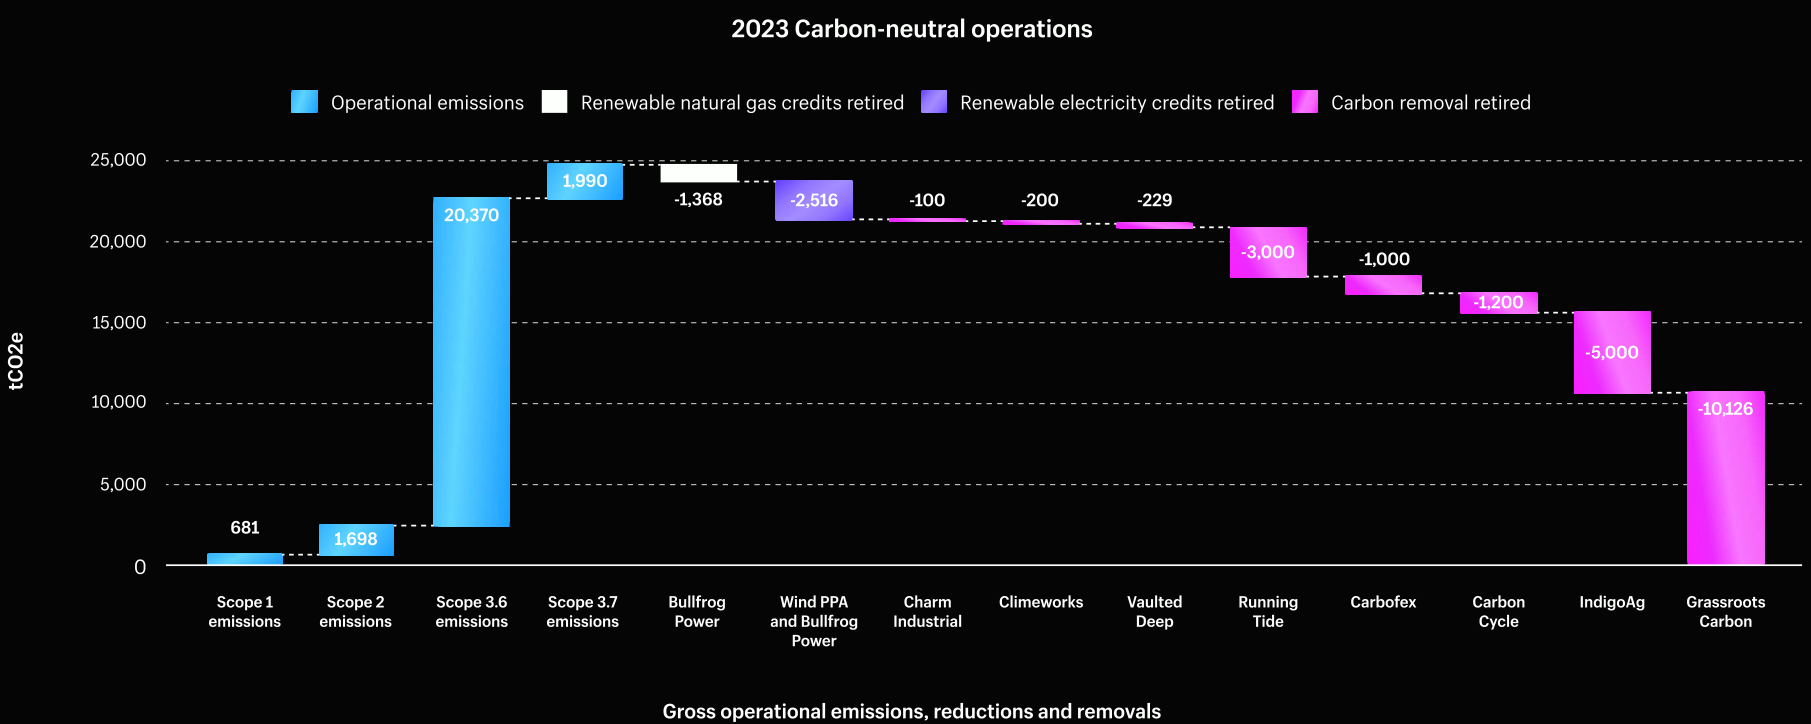
\includegraphics[width=0.9\textwidth]{images/ghg_emissions_bar_chart.png}
        \caption{Financial report page 1}
        \label{fig:financial_report_1}
    \end{subfigure}
    \begin{subfigure}{0.45\textwidth}
        \centering
        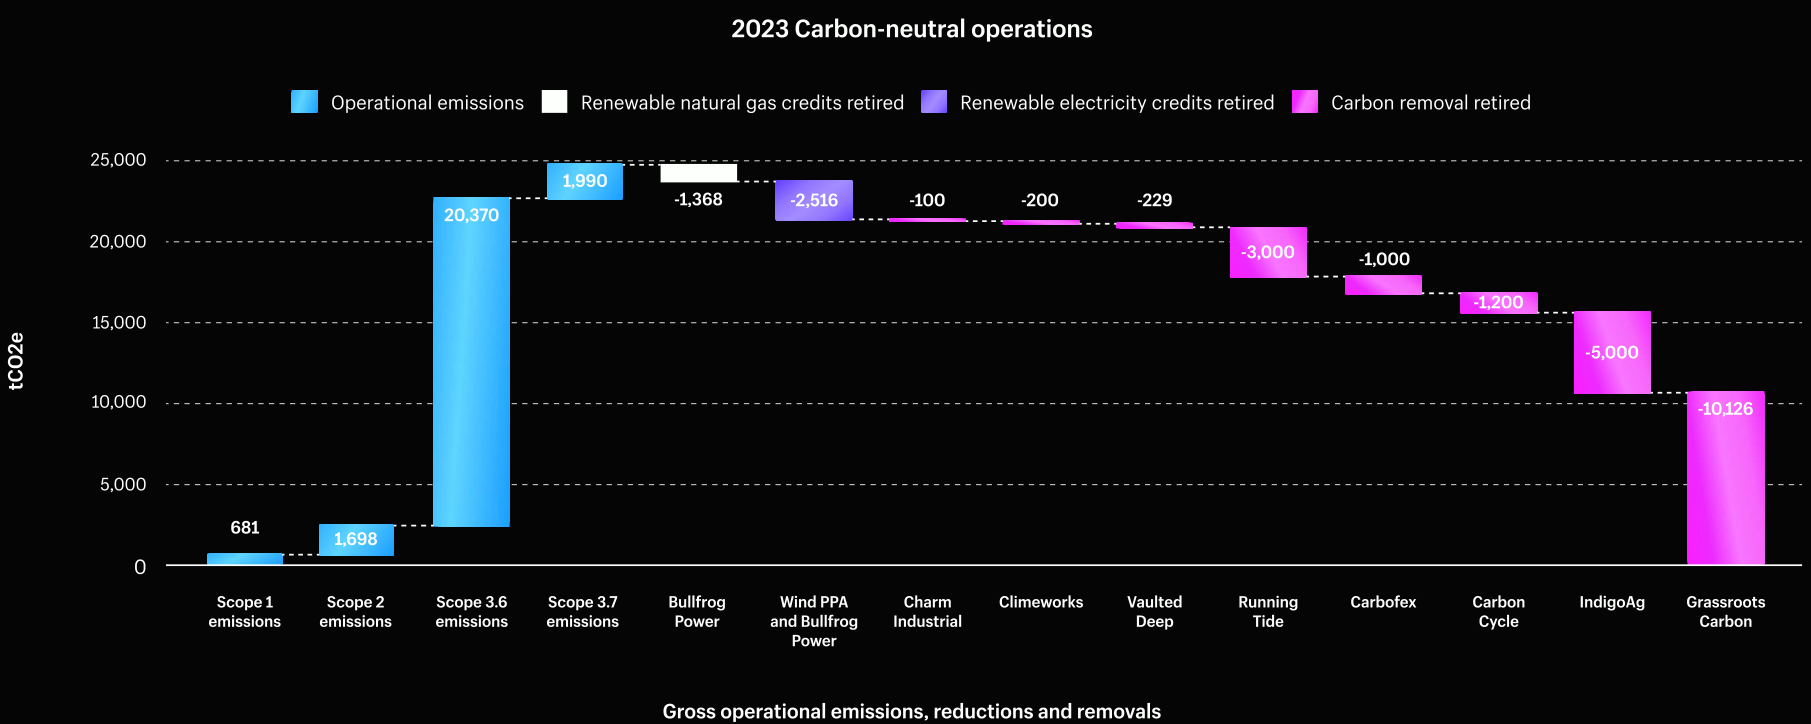
\includegraphics[width=0.9\textwidth]{images/ghg_emissions_bar_chart.png}
        \caption{Financial report page 2}
        \label{fig:financial_report_2}
    \end{subfigure}
    \begin{subfigure}{0.45\textwidth}
        \centering
        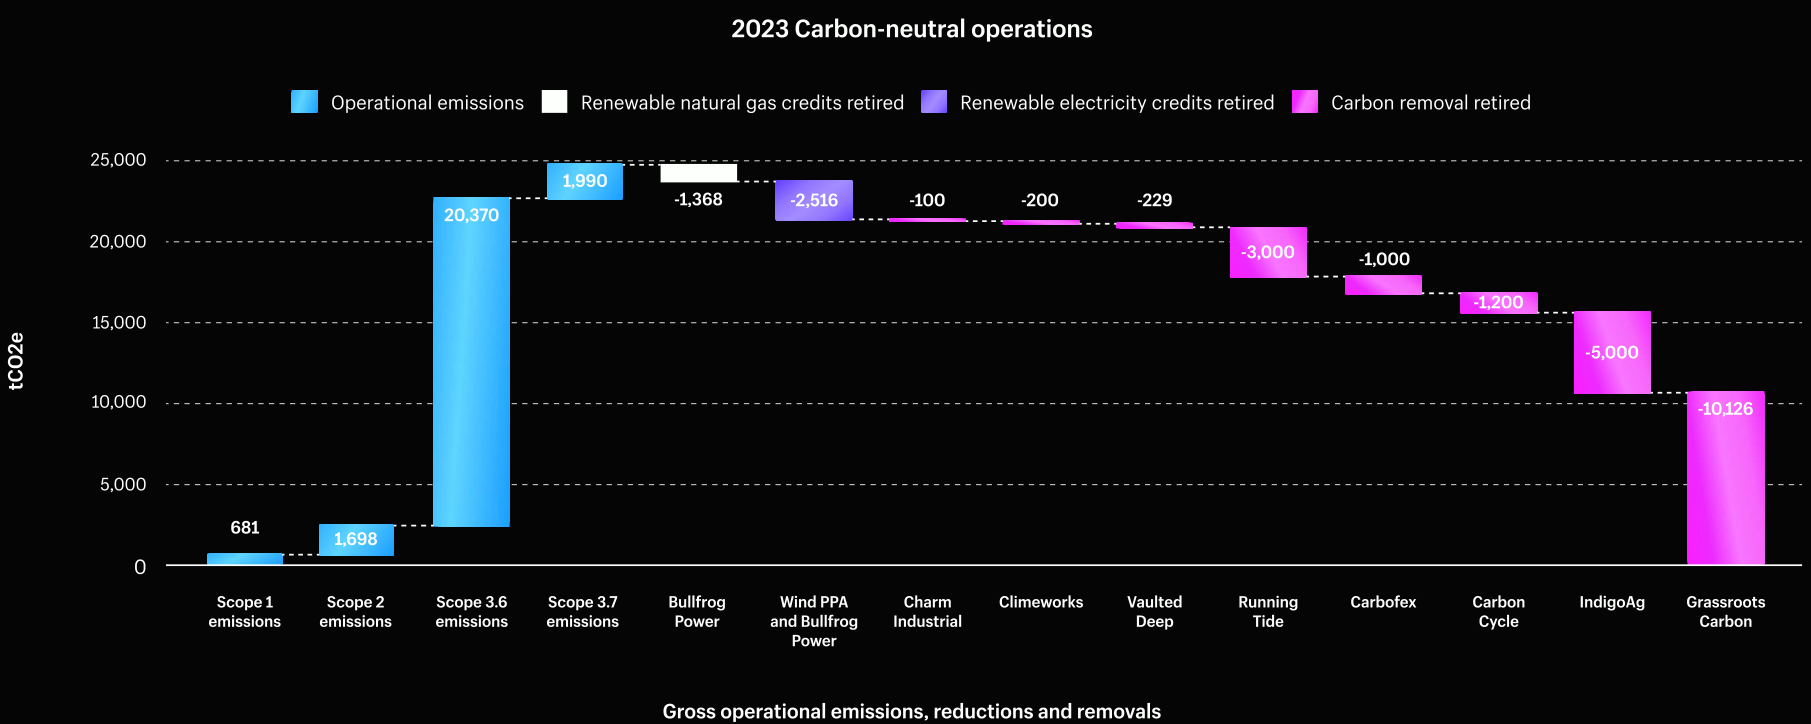
\includegraphics[width=0.9\textwidth]{images/ghg_emissions_bar_chart.png}
        \caption{Financial report page 3}
        \label{fig:financial_report_3}
    \end{subfigure}
    \caption{Sample pages from the financial reports dataset}
    \label{fig:financial_reports}
\end{figure}

\clearpage

\section{Strategies for information extraction from financial reports}

Different strategies for extracting information from financial reports have been implemented in order to compare their effectiveness across diverse report formats and content types.
The study brings a strategy that is focused solely on text information, an image-analysis approach that extracts information from images contained in the reports, and a multimodal approach that combines image and text information to validate extracted data from more than one source of truth.
For these different experiments, we consider that the core engine changes, but we maintain the same pre-processing steps across them to ensure that the comparison only takes into account the core feature of extracting data from a given input.

\subsection{System Specifications}

The experiments proposed in this study were conducted on a machine with the following specifications:

\begin{itemize}
    \item \textbf{CPU}: AMD Ryzen 7 3700X 16 threads at 3.600 GHz
    \item \textbf{Memory}: 32GB at 3200 MHz
    \item \textbf{Operating System}: Linux Manjaro 6.1.55-1
    \item \textbf{Python}: 3.11.5
\end{itemize}

\subsection{Experiments definition}

For the sake of setting up an \ac{OCR} challenge that that is relevant to business cases and provides the opportunity to compare different strategies for extracting information from financial reports, we establish a simple set of indicators of interest, a desired schema for the extracted data, and a set of metrics to evaluate the performance of the different strategies.

\subsubsection{Indicators of interest}

Given Datia's strong presence in the \ac{ESG} domain, we have chosen to focus on a set of \ac{ESG} indicators that are commonly reported in financial statements.
Therefore, this challenge focuses on correctly extracting values for the following indicators:

\begin{itemize}
    \item \textbf{\ac{GHG} Scope 1 emissions}: The total amount of \ac{GHG} emissions directly produced by a company.
    \item \textbf{\ac{GHG} Scope 2 emissions}: The total amount of \ac{GHG} emissions indirectly produced by a company.
            \begin{itemize}
                \item \textbf{Location-based}: Emissions calculated based on the location of the company's operations.
                \item \textbf{Market-based}: Emissions calculated based on the market where the company sells its products.
                \item \textbf{Undefined}: Emissions that are not clearly defined as location-based or market-based.
            \end{itemize}
    \item \textbf{\ac{GHG} Scope 3 emissions}: The total amount of \ac{GHG} emissions produced by in the value chain of a company.
    \item \textbf{Reported unit}: The unit of measurement used for the emissions.
\end{itemize}

These are crucial indicators for assessing a company's environmental impact and sustainability practices, and they are often reported in financial statements as part of the company's \ac{ESG} disclosures.
It's also important to be able to extract the unit of measurement used for the emissions, because different companies may report their emissions in different units, such as metric tons of \ce{CO2} equivalent, kilograms of \ce{CO2}, or other units.

\subsection{Extracted data schema}

The extracted data from the financial reports should follow a specific schema to ensure consistency and comparability across different strategies.
Since most of the strategies are \ac{LLM}-based, defining a schema adds complexity to the system, as hallucination could lead to correct data being extracted but in the wrong format.
For these reasons, we define a schema that is simple and straightforward, focusing on the key indicators of interest and their values for each year reported.
Here is an example of the \ac{JSON} schema for the extracted data:

\begin{minted}{json}
{
    "metrics": {
        "2022": {
            "scope_1": 88200000.0,
            "scope_2": {
                "location_based": null,
                "market_based": null,
                "undefined": 200000.0
            },
            "scope_3": 38800000.0
        },
        "2023": {
            "scope_1": 75100000.0,
            "scope_2": {
                "location_based": null,
                "market_based": null,
                "undefined": 200000.0
            },
            "scope_3": 36600000.0
        }
    },
    "extracted_pages": [1, 4, 10],
    "reported_unit": "million_metric_tonnes",
}
\end{minted}

This schema guarantees that the extracted data can be processed by the system and also be represented in the same unit of measurement, ensuring that the comparison between the different strategies is fair and accurate.
The \texttt{extracted\_pages} field is used to store the page numbers from which the data was extracted, allowing for traceability and validation of the extracted information.

\subsection{Evaluation Criteria}

To thoroughly assess the performance of the proposed systems for extracting indicators from financial reports, a combination of quantitative and qualitative metrics is employed.
These metrics are designed to measure both the accuracy of the extracted data and the robustness of the extraction process against various types of errors.
Here, we delineate the key metrics and evaluation criteria used.

\subsubsection{Precision and Recall}
Precision and Recall are critical metrics for evaluating the effectiveness of the data extraction system:
\begin{itemize}
    \item \textbf{Precision} assesses the proportion of data points extracted by the model that are correct and relevant. A high precision rate indicates fewer instances of fabricated metrics and irrelevant data extraction.

    \begin{equation}
        \text{Precision} = \frac{\text{True Positives}}{\text{True Positives} + \text{False Positives}}
    \end{equation}

    \item \textbf{Recall} measures the system's ability to retrieve all relevant data points from the document. High recall is essential to ensure no significant data is missed.

    \begin{equation}
        \text{Recall} = \frac{\text{True Positives}}{\text{True Positives} + \text{False Negatives}}
    \end{equation}
\end{itemize}

% Add formula for precision


% \subsubsection{F1 Score}
% The F1 Score is the harmonic mean of precision and recall, providing a single measure to balance these metrics. It is especially useful when the costs of false positives and false negatives are similar.

\subsubsection{\ac{MAPE}}

For numerical errors, the \ac{MAPE} is used to quantify the accuracy of the extracted values.
This metric calculates the average percentage difference between the extracted values and the ground truth values, providing insights into the model's performance in capturing the correct numerical data while accounting for scale and magnitude differences.

\begin{equation}
    \text{MAPE} = \frac{1}{n} \sum_{i=1}^{n} \left| \frac{y_i - \hat{y}_i}{y_i} \right| \times 100
\end{equation}

\subsubsection{Error Types Analysis}

In addition to quantitative metrics, an error analysis is conducted to identify the types of errors made by the system during the extraction process.

\begin{itemize}
    \item \textbf{Missing Data}: Indicates data that should have been extracted but was not. This error impacts the \texttt{recall} metric.
    \item \textbf{Incorrect Values}: Reflects errors in the value of the data extracted. These are numerical errors that impact the \texttt{MAPE} metric.
    \item \textbf{Fabricated Metrics}: Metrics that are not present in the document but appear in the extracted output --- also referred to as extrinsic hallucination. This error impacts \texttt{precision}.
\end{itemize}

\subsection{Common processing steps}

For all of the experiments, the system receives a \ac{PDF} as input and common pre and post-processing steps are applied to the data to ensure that the system is able to extract the information from the reports.

\subsubsection{Pre-processing: finding pages of interest}

A common pre-processing step is to find the pages of interest --- those that might contain the information that we are looking for --- in the \ac{PDF} document.

\begin{minted}{python}
def extract_data_from_pdf(pdf_file: str):
  # Load the PDF file
  doc = fitz.open(pdf_file)

  for page in doc:
    # extract text from page
    text = page.get_text("text")

    # function that will look for matches
    # for the indicators of interest
    matches = search_for_keywords(text)

    # this page does not contain
    # any relevant information
    if matches is None:
        return

    # Then different strategies follow...
\end{minted}

This pre-processing step is used to iterate over the pages in the \ac{PDF} document and find the pages of interest so that the core engine is only applied to these pages.
This is an important step to reduce the processing time and to avoid unnecessary processing of pages that do not contain relevant information, however it is also crucial to make sure that no false negatives are generated, as this could lead to missing pages of interest.

\subsubsection{Parsing \ac{LLM} outputs}

As of the time of writing, the text \ac{GPT}-4 model has a parameter flag to determine the output format of the model while the vision model does not have this feature.
This means that for text, it is possible to specify \ac{JSON} as the output format, however for the vision model, the output is always a string and that leads to uncertainty whether the output string can be parsed into a \ac{JSON} format by the system.
Additionally, the parameter flag does not guarantee that the output \ac{JSON} will contain the correct keys and meet the desired schema.
For these reasons, it is important to have a parsing step that validates the output of the \ac{LLM} models and ensures that the extracted data is in the expected format.

This is where the \textit{pydantic} and \textit{instructor} library comes into play, as we can use \textit{pydantic} to define the model schema and validate fields and types, and \textit{instructor} will handle any imperfections in the model by retrying the generation process $n$ times and validating the output against the defined schema.

% draw the diagram here


\subsubsection{Post-processing: consolidating information from different pages}

In an ideal world, all the information that we are looking for would be contained in one and only one page of the \ac{PDF} document and our system would be able to find the page, extract and return.
However, this is not the case in practice, as different companies choose different designs to display their information and sometimes the indicators are spread across different pages, or even repeated in different sections of the report.
Since our system needs to be able to resolve conflicts in the scenario of having multiple pages with the same information (potentially with different values due to different local regulations, units, and so forth), a strategy for consolidating the information is needed.
After testing out different strategies like frequency bags, picking the output with most found values, and \ac{LLM}s, we have decided to stick with the \ac{LLM}-approach by using \ac{GPT}-4 model, to consolidate the information from different pages.
Here is a demonstration of how this can be done:

\begin{minted}{python}
def consolidate_data(data: list[str]) -> str:
  """
  Consolidate data from different pages

  Args:
    data: List of JSON strings containing the data
          extracted from different pages

  Returns:
    consolidated_data: Unique JSON string containing
                       the consolidated data
  """
  # Send request with data and instructions to GPT4
  consolidated_data = openai.chat.completions.create(
    model="gpt-4-turbo-preview",
      response_format={"type": "json"},
      messages=[
        {
          "role": "system",
          "content": """Consolidate the following data
                        into only one JSON string...""",
        },
        {"role": "user", "content": data},
      ]
    )
  return consolidated_data
\end{minted}

This is a simple example of how the \ac{GPT}-4 model can be used to consolidate information from different pages of the \ac{PDF} document and can definitely be improved by adding more context and validation steps, such as checking for inconsistencies in the data, before returning the consolidated information.


\subsection{Text-only approach with \ac{LLM}s}

In this experiment, we use the \ac{GPT}-4 architecture, more especifically \textit{gpt-4-0125-preview} released in December 2023, to extract information from the text contained in the financial reports without considering any images or visual data.
Evidently, this approach is limited to the information that is present in the text and does not take into account any charts or important visual cues that the report might contain, thus it is expected that this system may fail for cases where the indicator are presented in a visual form.

\subsection{Image-only approach with \ac{LLM}s}

In this experiment, we use the \ac{GPT}-4 Vision model to extract information from the images contained in the financial reports without considering any text data.
Since OpenAI's visual model is highly accurate in extracting information from images, this approach is expected to have an overall performance superior to the text-only approach because it will be able to generalize the information from images but it is also expected to have an increased proclivity to hallucinations, as the model is not able to validate the information extracted from the images with the text data.

For this experiment, after the preprocessing step, for each of the pages of interest, the system applies the following image-processing transforms:

\begin{itemize}
\label{list:image_transforms}
    \item \ac{DPI}: The image is set to 300 \ac{DPI} to ensure that the model can extract the information with high quality. This setting has shown to be one of the optimal settings for \ac{OCR} tasks \cite{ocr_preprocessing2007}.
    \item Grayscale: The image is converted to grayscale to reduce the amount of information that the model needs to process.
    \item Downscaling: The image is downscaled such that they fit OpenAI's \ac{GPT}-4 Vision criteria:
    \begin{quote}
        \textit{...images are first scaled to fit within a 2048 x 2048 square, maintaining their aspect ratio. Then, they are scaled such that the shortest side of the image is 768px long \cite{OpenAIVisionAPI}.}
    \end{quote}
    \item Compression: The image is compressed to a 90\% quality to significantly reduce the size of the image while keeping sufficient quality for image analysis.
\end{itemize}

These transforms have the goal of reducing the amount of information that the model needs to process, while maintaining the quality of the information extracted from the images.
This is important not only for model performance, but also to keep the number of tokens processed lower, reducing the cost of the operation.

The system sends a request to OpenAI's \ac{GPT}-4 Vision model with the pre-processed image and the instructions where the model is asked to extract the key indicators from the image into a predefined JSON schema.
This is necessary and important because not only does the model need to be able to extract the information from the images, but it also needs to produce the information in a format that can be parsed by the system, otherwise it might raise unexpected errors on the client side.

\subsection{Multimodal \ac{LLM}s to extract information from images and text}

In this experiment, we use a multimodal approach to extract information from the financial reports, leveraging information from both textual and visual domains.
This approach combines the strengths of the text-only and image-only methods while mitigating their respective weaknesses by validating the information extracted from the images with the text data and vice versa.

The system follows the same pre-processing steps as the image-only approach before \ref{list:image_transforms} sending the image and instructions to the \ac{GPT}-4 Vision model.
The difference for this experiment is that the system also extracts the text from the page and creates a set of all the numbers mentioned in the page, which will be used to validate if the information given by the model is consistent with the text data or if it is an extrinsic hallucination.

In order to mitigate intrinsic and extrinsic hallucinations, we implement a simple lookup method that will search for the closest value in the text data to the one extracted from the image that is within a threshold limit so that the values that are within the threshold are considered valids and are readjusted while the ones that are not are considered hallucinations and are discarded.

This system is expected to have the best performance among the three approaches, as it is able to validate the information extracted from the images with the text data and vice versa, however it is also expected to have the highest processing time due to the increased complexity of the system.
% TODO Mention the behaviour noticed from hallucinations. i.e. erroring the last digits

\clearpage
\section{Results}


\subsection{Limitations of the dataset}

\subsection{Limitations of the data extraction systems}

Explain what are the observed limitations

\clearpage

\section{Conclusions}
\label{sec:summary}


\clearpage
%% Bibliography/ list of references
%%
\thesisbibliography

%reference bib file
\bibliographystyle{IEEEtranDOI}
\bibliography{references}

%% Appendices
%% If you don't have appendices, your thesis ends here. Remove \clearpage,
%% \thesisappendix and the following text below. The last command of this file
%% is \end{document}.
\clearpage

\thesisappendix

\section{Contents of an appendix}
\label{app:contents}

\end{document}
